\section{Introduction}

\begin{figure}[t]
    \centering
    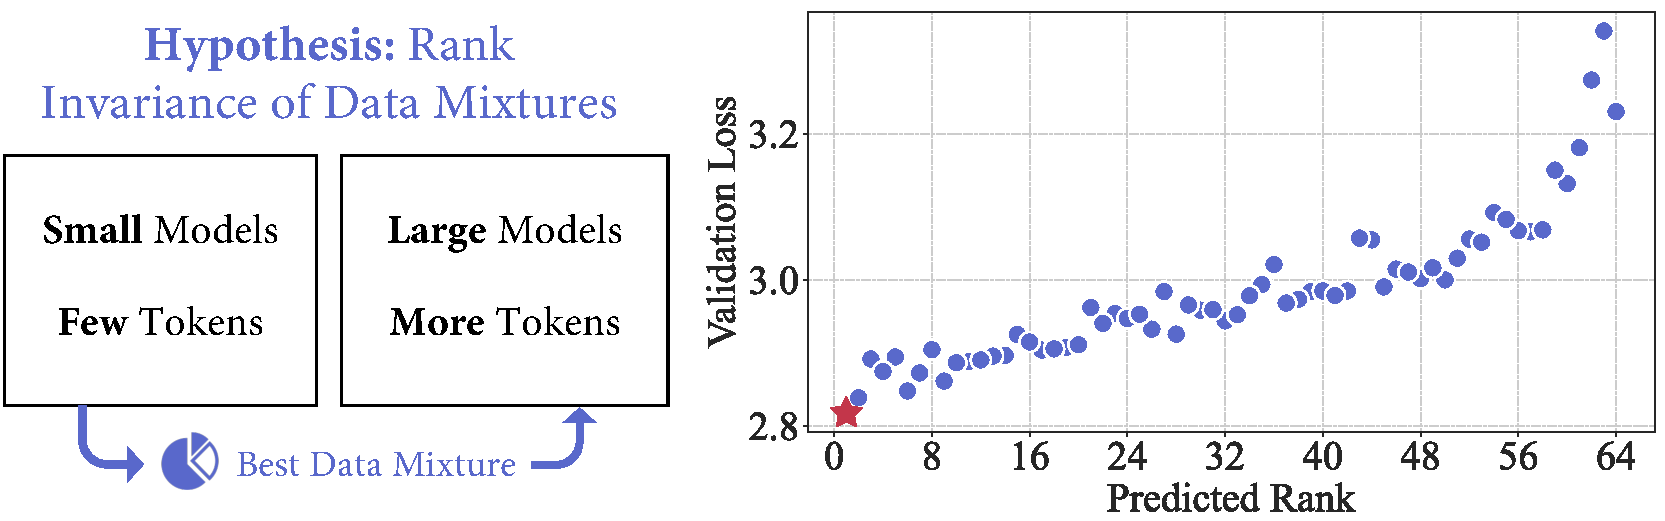
\includegraphics[width=1.0\textwidth]{figures/figure_1_overview.pdf}
    \caption{\textbf{Left}: We hypothesize the rank invariance of data mixtures across model sizes and numbers of training tokens. Leveraging this hypothesis, we use small models trained on fewer tokens to predict the effective data mixture for training large models with substantially more tokens. \textbf{Right}: By training $512 \times$ 1M models, our method identifies the best data mixture prior to training $64 \times$ 1B models. The predicted best data mixture, denoted by the red star, achieves the lowest validation loss.}
    \label{fig:1M_to_1B}
\end{figure}

The availability of large-scale public datasets has been a key factor enabling the creation of large language models (LLMs). Most data is available on the Internet and includes academic papers (e.g. arXiv), books (e.g. Project Gutenberg), and code (e.g. GitHub). For the creation of one of the first LLMs, GPT-3~\citep{gpt3paper}, the authors had already recognized the importance of selecting the best data for training, and thus they decided to upsample Wikipedia due to its perceived high quality. However, such manual data selection is not scalable and may lead to a suboptimal selection~\citep{albalak2024survey}.
As the size and diversity of data used for LLM pre-training continue to grow, determining the optimal data mixture becomes increasingly challenging.
It gives rise to the critical research question: \textit{How can we select the optimal data mixture in a scalable and efficient manner?} \looseness=-1

Prior work~\citep{xie2023doremi,fan2023doge,albalak2023efficient} employs small-scale models (``proxy models'') to predict the domain weights for large-scale language models. These works train proxy models with a substantial number of tokens (e.g., 100B), sometimes even the same number as used for training LLMs, and dynamically adjust the data allocation strategy by monitoring the training dynamics. However, these approaches become inefficient as the training data used for pre-training LLMs continues to grow.
Training a proxy model for current models, such as Llama-3, would require using up to 15T tokens~\citep{meta_llama_3_2024} with current approaches, which is likely too expensive and too slow to make it worthwhile~\footnote{These approaches often suffer from instability issues. Details can be found in Appendix~\ref{appendix:stability}.}.

In this work, we argue that \textit{training small models on a limited set of tokens} is sufficient to predict an effective data mixture for LLM training. Our key assumption is the \textit{rank invariance of data mixtures}, which posits that the relative ranking of data mixtures in terms of their impact on model performance is consistent across different model sizes and numbers of training tokens. Under this assumption, the key challenge lies in discovering the top-ranked data mixture from the near-infinite number of potential data mixtures. To do so, we treat the data mixture selection as a regression task. Rather than exhaustively training small models with every possible mixture, we train only a set of small models, each with a unique data mixture. Based on the performance of these models and their mixtures, we fit a regression model to predict the performance of other data mixtures. Our approach is significantly more scalable than prior work, as it allows for parallel training of small proxy models rather than training a single model for a long time. Further, the regression model provides insights into domain interactions that can facilitate understanding and data curation.  \looseness=-1

To validate \ourmethod, we train models with 1M and 1B parameters\footnote{Our model sizes mentioned in this paper refer to the number of non-embedding parameters, as embedding parameters account for a disproportionately large portion in smaller models.} with different data mixtures. By training 512 models with 1M parameters on 1B tokens\footnote{The estimated FLOPs for training $512 \times$ 1M models is nearly 2\% of the FLOPs required for one 1B model.}, we are able to predict the optimal data mixture among 64 models that are $1000 \times$ larger (1B parameters) and trained $25 \times$ longer (25B tokens) as depicted in Figure~\ref{fig:1M_to_1B}.
Moreover, the optimized data mixture using \ourmethod yields a better model than human selection, and achieves performance on par with the flagship DoReMi method~\citep{xie2023doremi} despite it requiring less total compute and allowing for parallel training.
We also find that (1) Data mixture significantly impacts downstream performance, resulting in substantial differences of up to 14.6\% in single-task performance; (2) General web corpora (e.g., CommonCrawl), rather than Wikipedia, exhibit the strongest positive correlation with improved performance across downstream tasks;
(3) The interactions between domains are complex and often contradict intuition, highlighting the need for automated approaches like \ourmethod. (4) Data mixture effects transcend scaling laws, and \ourmethod captures the complexity by considering all domains together. \looseness=-1
